% this file is called up by thesis.tex
% content in this file will be fed into the main document

%: ----------------------- name of chapter  -------------------------
\chapter{Phương pháp giải quyết} % top level followed by section, subsection


%: ----------------------- paths to graphics ------------------------

% change according to folder and file names
\ifpdf
    \graphicspath{{3/figures/PNG/}{3/figures/PDF/}{3/figures/}}
\else
    \graphicspath{{3/figures/EPS/}{3/figures/}}
\fi

%: ----------------------- contents from here ------------------------


\noindent Chương này chúng tôi sẽ trình bày về hệ thống theo dõi tin tức trực tuyến có tên $\mathcal{N}$\texttt{ewSOMoni}
\footnote{[nju: 's$\Lambda$m m$\Lambda$ni]} \footnote{$\mathcal{N}$\texttt{ew} \overbrace{S}^{\mbox{Smartness}} \underbrace{O}_{\mbox{Orientation}} \overbrace{M}^{\mbox{Magnitude}}oni \hspace{0.2in}   \mbox{viết tắt của \texttt{News Online Monitoring}}} cùng  phương pháp lai giữa luật và học máy Maximum Entropy trong pha trích xuất sự kiện của hệ thống vừa được nhắc tới. Trước tiên, mô hình đề xuất và diễn giải chi tiết hệ thống được thể hiện ở phần \ref{system} ngay dưới đây. Sau đó, phương pháp lai trích xuất sự kiện được nói tới  ở phần \ref{method} (trang \pageref{method}).




\section{Hệ thống theo dõi tin tức trực tuyến  $\mathcal{N}$\texttt{ewSOMoni}}
\label{system}
%\figuremacro{largepotato}{Mô hình hệ thống}{ok}}
%\figuremacro{system}{Mô hình hệ thống}}
\noindent Công trình nghiên cứu này chúng tôi đã xây dựng một hệ thống theo dõi tin tức trực tuyến. Nhiệm vụ chính của hệ thống là quan sát tức mới được đưa lên các nguồn cung cấp tin tức (phụ lục \ref{website}, trang \pageref{website}), phân loại và nhận dang sự kiện thuộc ba lĩnh vực: \textsc{Tai nạn giao thông}, \textsc{Hình sự}, \textsc{Cháy nổ}. Cuối cùng là trực quan hóa trên bản đồ cho người dùng dễ dàng theo dõi, cập nhật. \\
\noindent Mô hình của hệ thống được thể hiện rõ ở hình \ref{system}. Hệ thống $\mathcal{N}$\texttt{ewSOMoni} có bốn phần chính:
\begin{itemize}
  \item \textbf{Data Crawler} thu thập dữ liệu tự động và tiền xử lý dữ liệu
  \item \textbf{NoSQL--Database} cơ sở dữ không ràng buộc, hướng tài liệu (MongoDB), lưu trữ lượng  lớn dữ liệu tin tức
  \item \textbf{Event Extracter} thực hiện các bước cần thiết để trích xuất sự kiện
  \item \textbf{Visual Interface} có nhiệm vụ tương tác với cơ sở dữ liệu để hiển thị thông tin cho người dùng

  \end{itemize}

\noindent Mỗi thành phần của hệ thống sẽ được diễn giải chi tiết ngay dưới đây.

\subsection{Data Crawler}
\label{datacrawler}




\subsection{NoSQL--Database}
\label{db}

\subsection{Event Extracter}
\label{ee}


\subsection{Visual Interface}
\label{vi}






\begin{figure}[htbp]
		\centering
		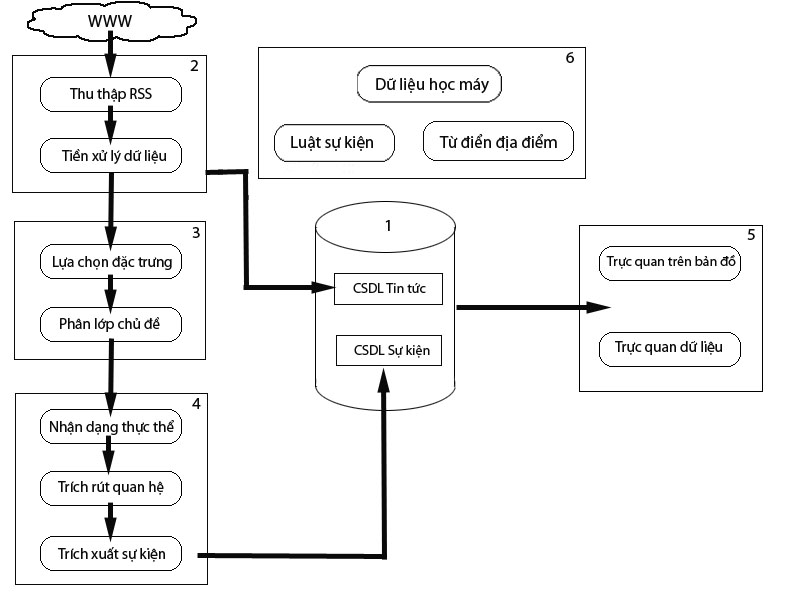
\includegraphics[width=1\textwidth]{system}
		\caption{\textbf{Mô hình hệ thống  $\mathcal{N}$\texttt{ewSOMoni}}}
		\label{system}
\end{figure}




\section{Kết hợp luật và Maximum Entropy trong trích xuất sự kiện}
\label{method}

% ---------------------------------------------------------------------------
%: ----------------------- end of thesis sub-document ------------------------
% ---------------------------------------------------------------------------
